\chapter{Bitcoin}
\label{chap:bitcoin}

\section{Introduzione}
\label{sec:introduzione}

Bitcoin introdusse per primo il concetto di blockchain: ciò permise la creazione di un metodo di pagamento peer-to-peer esente da un intermediario, definito anche come criptovaluta decentralizzata.
Introdotto da una persona o un gruppo di persone sotto lo pseudonimo di \say{Satoshi Nakamoto}, Bitcoin viene descritto per la prima volta nel white paper intitolato \say{Bitcoin: A Peer-to-Peer Electronic Cash System} pubblicato nell’ottobre 2008 sulla mailing list di crittografia del sito \url{https://www.metzdowd.com}.\newline
Il 3 gennaio 2009 venne rilasciata la versione 0.1 del codice sorgente sotto licenza MIT da Satoshi Nakamoto che smise di contribuire al progetto nel dicembre 2011. Si stima che ad oggi Satoshi Nakamoto possegga un milione di bitcoin\footnote{Un milione di bitcoin equivale a 7,658,863,492.00 di euro, nel 16/11/2019}, sparsi in vari wallet.

\section{Transazioni}
\label{sec:transazioniBitcoin}

Le transazioni sono una parte fondamentale di Bitcoin. Infatti tutto il sistema è progettato per assicurare la creazione, propagazione e pubblicazione di transazioni su blockchain, ma queste ultime sono concettualmente differenti dalle transazioni a cui siamo abituati: ad esempio, una transazione di un database relazionale rappresenta un evento che innesca un cambio di stato all’interno della base di dati, dove in caso di malfunzionamenti la base di dati ritorna nella condizione precedente, prima che l’evento fosse scatenato.
Le transazioni di Bitcoin sono concettualmente differenti.


\begin{example}
\label{example:aliceBobFirst}
Consideriamo il seguente scenario con i seguenti personaggi:

\begin{itemize}
  \item Alice e Bob sono due utenti che usano attivamente Bitcoin per effettuare i loro pagamenti.
  \item Vincent è un partecipante della rete di Bitcoin e si occupa di effettuare il mining (argomento trattato nella Sezione \ref{sec:miningbitcoin}) per proteggere la rete e trarre ricavi in bitcoin.
\end{itemize}

Alice ha deciso di inviare 0.00700767 bitcoin a Bob; Alice dopo aver ottenuto l’indirizzo Bitcoin di Bob, che corrisponde a \say{33mMAc6nGyENdKMQTr5SrKoEkwNTeZQUx9}, può inviare dei bitcoin a Bob, generando una nuova transazione con il seguente identificativo: \say{ddd587d54b693a9bc9bda2218c6f5e17979f6ac53755c5c1f668f3fa728e472d}.\newline
Questa nuova transazione consuma una precedente transazione in possesso di Alice, chiamata UTXO (\emph{unspent transaction output}), e crea un nuovo UTXO in possesso di Bob; la nuova transazione viene verificata da un componente (nodo) della rete, in questo caso Vincent.

{\centering
\vspace{15pt}
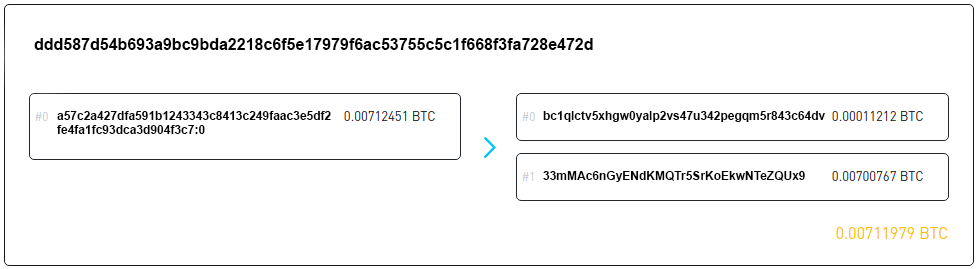
\includegraphics[scale=0.35]{images/example_alice_bob_vincent.png}
\captionof{figure}{La nuova transazione creata da Alice ricercata attraverso un explorer \cite{blockstream:esplora}.\label{fig:examplealicebob}}
\vspace{10pt}
\par}

Come illustrato in Figura \ref{fig:examplealicebob}, l'operazione di Alice provoca lo spostamento di bitcoin da una precedente transazione con il seguente identificativo: \say{a57c2a427d\-fa591b1243\-343c8413c249\-faac3e5df2fe4fa1fc93dca3d904f3c7} a due diversi indirizzi, cioè:

\begin{itemize}

  \item 33mMAc6nGyENdKMQTr5SrKoEkwNTeZQUx9 (indirizzo Bitcoin di Bob);

  \item bc1qlctv5xhgw0yalp2vs47u342pegqm5r843c64dv (indirizzo Bitcoin di Alice): poiché gli UTXO sono indivisibili, essi devono venire consumati interamente.  Nel momento in cui si genera una nuova transazione viene scelto l’UTXO più adatto con un valore di bitcoin uguale al valore da inviare a Bob; se questo non esiste, si seleziona l'UTXO \emph{best fit},  con la conseguenza che il wallet genererà una nuova transazione (conosciuta come \emph{exchange transaction}) verso se stesso per recuperare i bitcoin rimanenti. Questo processo è illustrato in Figura \ref{fig:examplechangeutxo}.


%  la motivazione della generazione di un UTXO verso Alice, che in questo esempio ha generato una nuova transazione per inviare bitcoin a Bob, è il seguente:  gli UTXO di Alice non vengono mischiati e messi insieme ma bensì gli UTXO sono unità indivisibili e vengono mantenuti separatamente come illustrato in Figura \ref{fig:examplechangeutxo}.

  \begin{figure}[h]
  \begin{center}
  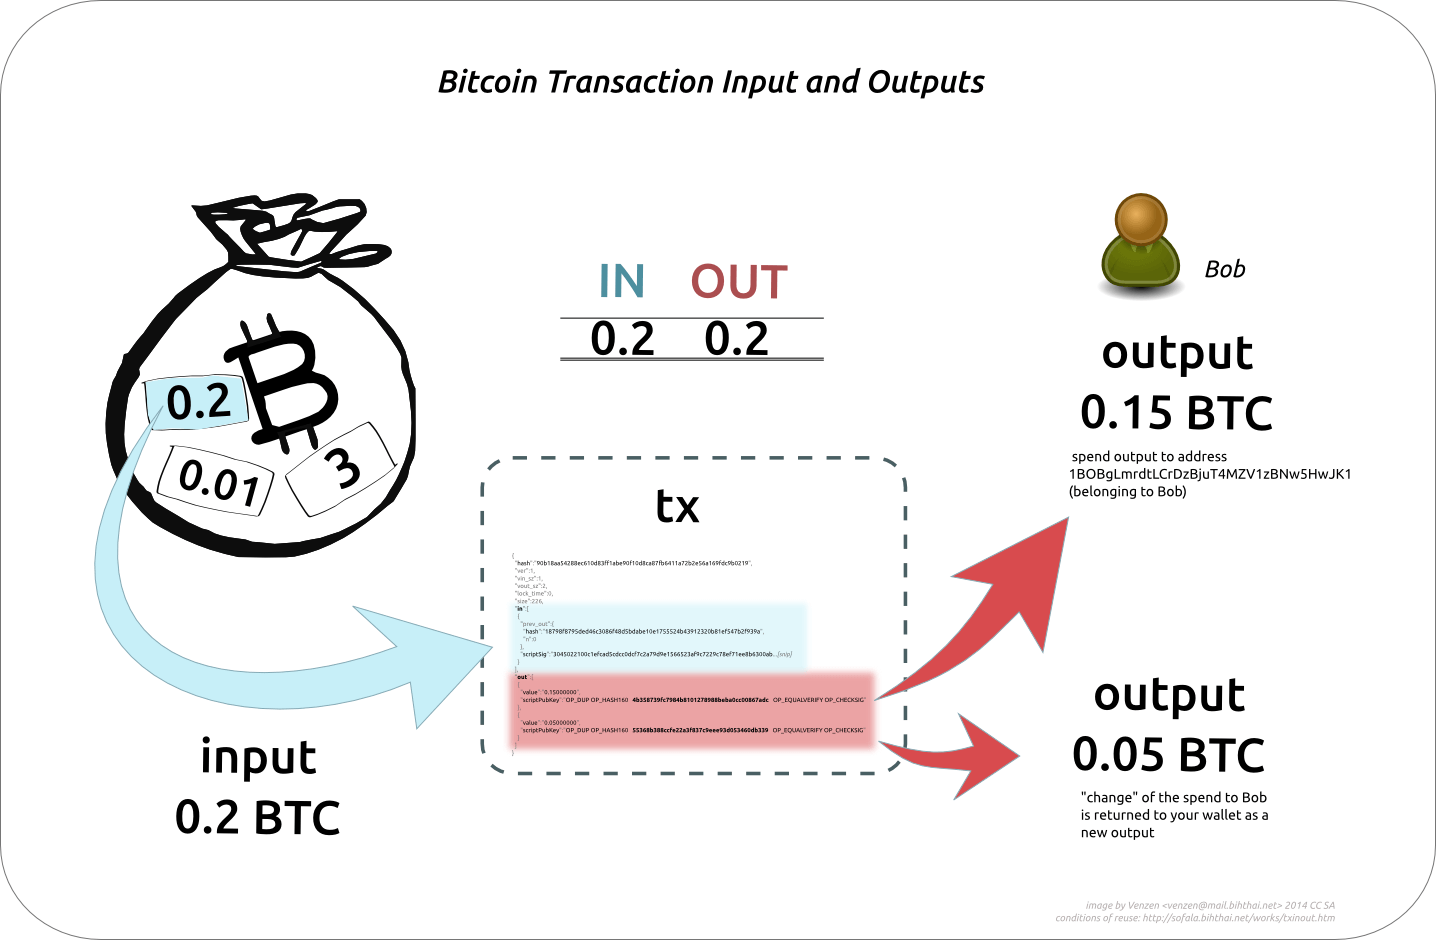
\includegraphics[width=0.6\columnwidth]{images/change_utxo.png}
  \end{center}
  \caption{Gestione degli UTXO nella blockchain di Bitcoin \cite{blockstream:esplora}.}
  \label{fig:examplechangeutxo}
  \end{figure}
%  Nel momento in cui si genera una nuova transazione viene scelto l’UTXO può adatto con un valore di bitcoin uguale al valore da inviare nella nuova transazione se questo non esiste si seleziona l’UTXO con un valore maggiore di bitcoin con la conseguenza che il wallet genererà una nuova transazione verso se stesso per recuperare i bitcoin rimanenti; come quanto si effettua un pagamento di 25 euro in un ristorante con una banconota da 50 euro in cui bisogna restituire 25 euro di resto.
%  \item 33mMAc6nGyENdKMQTr5SrKoEkwNTeZQUx9: Indirizzo Bitcoin di Bob.
\end{itemize}

La verifica della nuova transazione di Alice viene effettuata da Vincent, il quale inserisce la transazione in un nuovo blocco insieme a tutte le altre pubblicate sulla rete in quel momento.

Nel momento in cui viene pubblicato il blocco il sistema crea una transazione verso Vincent come premio per il lavoro svolto; questa nuova transazione è conosciuta con il nome di transazione \emph{coinbase} ed è mostrata in Figura \ref{fig:examplecoinbasetxvincent}.

{\centering
\vspace{15pt}
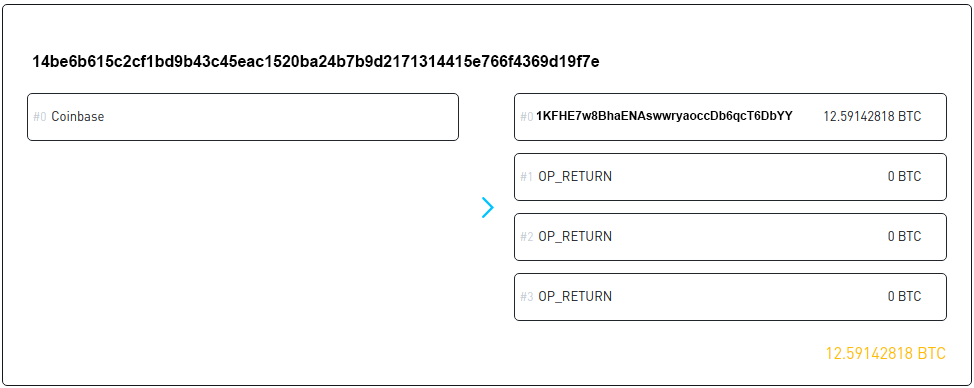
\includegraphics[scale=0.35]{images/example_coinbase_vincent.png}
\captionof{figure}{Transazione coinbase descritta  \cite{blockstream:esplora}.\label{fig:examplecoinbasetxvincent}}
\vspace{10pt}
\par}

\end{example}

L'esempio precedente mostra come  in Bicoin si possano distinguere due tipi di transazioni: la transazione {\it coinbase\/} e la transazione comune.
\begin{itemize}
  \item La transazione coinbase è un evento speciale che si verifica sul sistema, il cui formato risulta non valido per la blockchain, poiché la sua struttura contiene zero input e un output. Questo evento rappresenta nel sistema un’emissione di nuovi bitcoin (argomento trattato nella Sezione \ref{sec:miningbitcoin}), rendendo la transazione coinbase una transazione speciale per il sistema Bitcoin.
  \item Una transazione comune è un evento che punta a sbloccare una transazione esistente su blockchain, conosciuta come UTXO, allo scopo di   creare un movimento di bitcoin.
\end{itemize}

Possono verificarsi principalmente due tipi di fallimenti durante la creazione di una transazione:
\begin{enumerate}
  \item Una transazione non è valida per il sistema Bitcoin; in questo caso esso viene inoltrata alla rete come una transazione valida, ma essa verrà rigettata dal primo nodo completo\footnote{Per nodo completo viene inteso un nodo che possiede l’intera copia della blockchain ed è abilitato per la validazione di transazioni; esso viene utilizzato comunemente dai miner.} utile. Un esempio di transazione non valida è una transazione che contiene zero input ed un output.
  \item Una transazione valida per il sistema ma non valida per sbloccare UTXO: essa viene accettata dal sistema Bitcoin perché valida, ma la transazione non è capace di sbloccare nessun UTXO. Un esempio è costituito da  una transazione che prova a spendere due volte lo stesso UTXO (evento di doppia spesa).
\end{enumerate}
Bitcoin pertanto descrive le transazioni come \say{consumabili}, cioè una transazione di input consuma un UTXO e nello stesso istante produce un UTXO ex novo.
\begin{example}
Consideriamo nuovament l'esempio precedente  e supponiamo che Bob abbia deciso di inviare parte dei bitcoin ricevuti da Alice a Sara. Una volta ottenuto l’indirizzo Bitcoin di Sara, cioè \say{3CM8TuY8B3\-sCzVQN3FWYnd5skmzSF3uvWA}, per effettuare il trasferimento Bob  crea una nuova transazione di 0.00137927 bitcoin con il seguente identificativo \say{907538047d630d571298096028572\-08705ef3baa4b573e6e845d5a3e6ea\-11464}, raffigurata in Figura \ref{fig:examplebobsara}.

{\centering
\vspace{15pt}
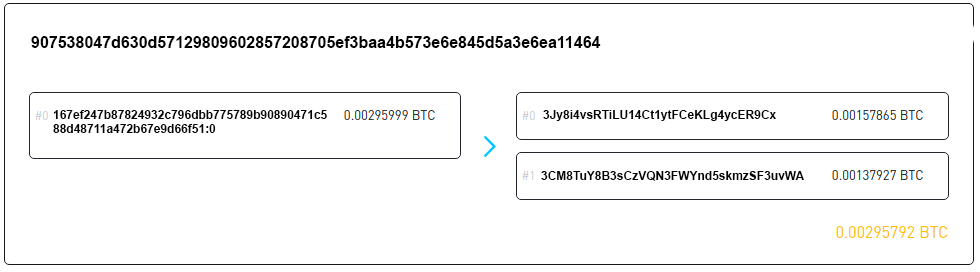
\includegraphics[scale=0.35]{images/example_bob_sara.png}
\captionof{figure}{La transazione creata da Bob verso Sara \cite{blockstream:esplora}.\label{fig:examplebobsara}}
\vspace{10pt}
\par}

%In questo scenario viene illlustrato il modo in cui Bob utilizza il suo UTXO per creare una nuova transazione verso Sara; come illustrato nella Figura \ref{fig:examplechangeutxo} gli UTXO non sono raggruppati ma quest’ultimi vengono contenuti all’interno di un'aria in cui risiedono tutti gli UTXO: quindi in questo esempio Bob deve fornire una prova che la transazione sia effettivamente sua, inoltre in seguito deve utilizzare un modo per cui Sara (solo lei) sarà in grado di spendere il suo UTXO.

Poiché gli UTXO sono contenuti all’interno di un'area in cui risiedono tutti gli UTXO, Bob deve fornire una prova che la transazione UTXO che vuole consumare sia effettivamente sua; inoltre in seguito deve utilizzare un modo per cui solo Sara  sarà in grado di spendere il suo UTXO.

A tale scopo Bitcoin offre un sistema di blocco delle transazioni di output e un sistema di sblocco per le transazioni di input.  Questo sistema si basa sull'impiego di script (argomento trattato nella Sezione \ref{sec:bitcoinScriptBitcoin}) che utilizzano estensivamente tecniche crittografiche con cui è possibile verificare la proprietà di quell'UTXO.
Nell'esempio in cui Alice crea una nuova transazione per Bob, per rendere la transazione sbloccabile solo da Bob, Alice ha inserito all’interno dello script di blocco dell’UTXO la chiave pubblica di Bob.\newline
Bob per creare una transazione verso Sara deve sbloccare l’UTXO che gli appartiene fornendo all’interno dello script di sblocco (contenuto all’interno la transazione di input) la firma della sua chiave privata e in un secondo momento deve creare un UTXO sbloccabile solo da Sara inserendo all’interno lo script di blocco la chiave pubblica di Sara.\newline
In Figura \ref{fig:lockunlockexample} viene rappresentato il flusso di eventi che descrive il blocco e sblocco di un UTXO.

{\centering
\vspace{5pt}
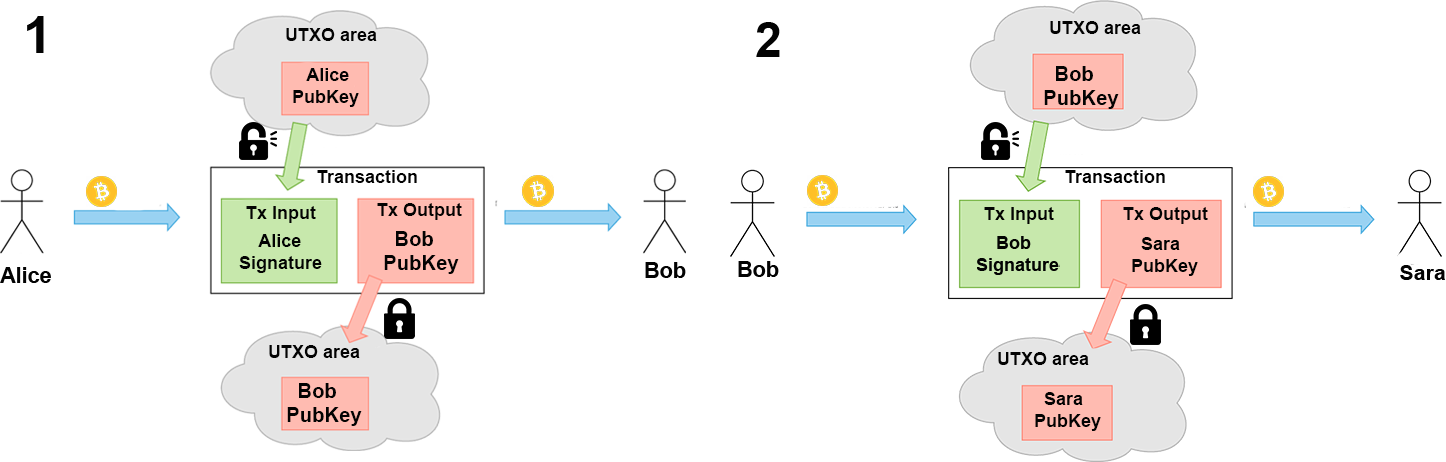
\includegraphics[scale=0.2]{images/DiagramUnlocLockUTXO.png}
\captionof{figure}{Rappresentazione del evento di blocco e sblocco di un UTXO.\label{fig:lockunlockexample}}
\vspace{10pt}
\par}

\end{example}

Bitcoin è il primo tentativo di successo ad introdurre il concetto di transazione come struttura dati che definisce un trasferimento di valore da una o più fonti ad una o più destinazioni.

\begin{table}[H]
       \centering\small
           \begin{tabular}{|c|}
               \hline
               \textbf{RawTransaction}\\
               \hline \hline
               Versione   \\
               \hline
               Transazioni di input \\
               \hline
               Transazioni di output \\
               \hline
               Lock time \\
               \hline
       \end{tabular}
       \caption{Struttura delle transazioni in Bitcoin.\label{tab:rawtransactionbitcoin}}
   \end{table}

La struttura della transazione (Tabella \ref{tab:rawtransactionbitcoin}) contiene dei campi che forniscono informazioni addizionali, ad esempio:
\begin{itemize}
  \item {\bf Versione\/}: indica le regole che strutturano la transazione.
  \item {\bf LockTime\/}: definisce il primo istante in cui la transazione viene considerata valida e può essere trasmessa sulla rete Bitcoin; è rappresentato attraverso un valore intero compreso tra 0 e 500 milioni, assumendo  significati diversi in base al valore assegnato, cioè:
  \begin{itemize}
    \item \(LockTime = 0 \): la transazione viene propagata ed eseguita all’istante di creazione.
    \item \( LockTime \in (0, 500\; milioni]\): il valore viene interpretato come un’altezza di blocco, cioè la transazione sarà valida solo dopo essere stato pubblicato il blocco con altezza uguale al valore di lock time.
    \item \(LockTime > 500\; milioni\): il valore viene interpretato come timestamp Unix e quindi la transazione sarà valida solo dopo la data rappresentata dal valore di lock time.
  \end{itemize}
\end{itemize}

Gli input di transazione e gli output hanno anche loro una struttura che definisce il  modo in cui si possono “spendere” i bitcoin associati a quella transazione; tale struttura contiene anche  altre informazioni addizionali, ma nessuna di esse è relazionata direttamente con un wallet oppure un’identità. \newline
La struttura delle transazioni di output (Figura \ref{tab:outputtransaztionbitcoin}) introduce un concetto fondamentale per Bitcoin, cioè le transazioni di output non spese, conosciute anche come UTXO.
Quasi tutte le transazioni di output sono UTXO riconosciute da tutta la rete Bitcoin e sbloccabili attraverso uno script di sblocco (scriptSig).

\begin{table}[H]
       \centering\small
           \begin{tabular}{|c|}
               \hline
               \textbf{Transazione di output}\\
               \hline \hline
               Importo   \\
               \hline
               Script di blocco (ScriptPubKey) \\
               \hline
       \end{tabular}
       \caption{Rappresentazione struttura delle transazioni di output.\label{tab:outputtransaztionbitcoin}}
   \end{table}

\begin{itemize}
  \item {\bf Valore\/}: valore di bitcoin espressi in satoshi che rappresentano una frazione di bitcoin come i centesimi per gli euro, \( 1\: bitcoin = 1*10^8 \: satoshi \).
  \item {\bf Script di blocco\/}: conosciuto come script \emph{public key}, contiene le informazioni necessarie per bloccare l’output e non permettere a chiunque di spenderlo.
\end{itemize}

La struttura delle transazioni di input (Tabella \ref{tab:inputtransaztionbitcoin}) contiene due informazioni importanti: il riferimento alla transazione precedente e la condizione di sblocco della UTXO.

\begin{table}[H]
       \centering\small
           \begin{tabular}{|c|}
               \hline
               \textbf{Transazione di input}\\
               \hline \hline
               Hash della transazione precedente   \\
               \hline
               Index della transazione di output \\
               \hline
               Script di sblocco (ScriptSig) \\
               \hline
               Sequence \\
               \hline
       \end{tabular}
       \caption{Rappresentazione struttura delle transazione di input in Bitcoin.\label{tab:inputtransaztionbitcoin}}
   \end{table}

\section{Bitcoin Script} \label{sec:bitcoinScriptBitcoin}

Gli script all’interno delle transazioni di Bitcoin vengono scritti in Bitcoin Script che è un linguaggio basato su stack e contiene molti operatori.\newline
La mancanza di loop e funzionalità di controllo di flusso complesse rende Bitcoin Script molto limitato rispetto a linguaggi moderni come Solidity; questo cataloga Bitcoin Script come un linguaggio di programmazione non Turing completo e garantisce così l’impossibilità di eseguire loop infiniti oppure fenomeni di code-injection all’interno delle transazioni, che potrebbero causare attacchi DoS (denial-of-service) sulla rete Bitcoin.\newline
Gli script vengono eseguiti in modalità atomica, cioè senza possedere uno stato pre e post esecuzione. Bitcoin convalida le transazioni eseguendo gli script contenuti al suo interno: in particolare lo script di sblocco e lo script di blocco vengono eseguiti in sequenza e l'input risulta valido solo nel caso in cui lo script di sblocco soddisfi le condizioni dello script di blocco.

Nel client Bitcoin originale, gli script di sblocco e blocco venivano concatenati ed eseguiti in sequenza, ma per motivi di sicurezza questo è stato modificato nel 2010, a causa di una vulnerabilità che ha permesso a uno script di sblocco non valido di inviare dati nello stack e corrompere lo script di blocco.
Nell'attuale implementazione, gli script vengono eseguiti separatamente, con lo stack trasferito tra le due esecuzioni, dove è possibile dividere la modalità di esecuzione in due passi:

\begin{enumerate}
  \item Lo script di sblocco viene eseguito: se l’esecuzione non riporta errori, allora lo stack principale viene copiato e lo script di blocco viene eseguito.
  \item Se, eseguendo lo script di blocco con i dati dello stack precedente, nel nuovo stack il risultato è \say{TRUE}, allora lo script di sblocco è riuscito a risolvere le condizioni imposte dallo script di blocco e, pertanto, l'input è un'autorizzazione valida per spendere UTXO. Se dopo l'esecuzione dello script combinato rimangono risultati diversi da \say{TRUE}, l'input non è valido perché non è riuscito a soddisfare le condizioni di spesa inserite in UTXO.
\end{enumerate}

Durante lo sviluppo sono state rese possibili l’esecuzione di soli script di transazioni standard: ad oggi l’implementazione di riferimento ne contiene sette e sono definite in un tipo enumerazione all’interno del file {\tt{standard.h}} (Codice \ref{code:enumtx}) del client Bitcoin Core.

\lstinputlisting[language=C++, label=code:enumtx, caption=Porzione di codice che riporta il tipo enumerazione nel file standard.h di bitcoin core.]{code/enumtx.cpp}

\subsection{P2PKH}
Lo script {\it pay-to-public-key-hash \/} fino a qualche anno fa era la tipologia di script più diffusa, perché lo script di blocco veniva composto dal hash della chiave pubblica e questo consentiva di non esporre la chiave pubblica del ricevente; l’output può essere sbloccato da uno script di sblocco contenente la chiave pubblica e la firma. Un esempio generalizzato potrebbe essere il seguente:

\begin{lstlisting}[language=bitcoinscript, caption={P2PKH Script di blocco.}]
 OP_DUP OP_HASH160 <A Public Key Hash> OP_EQUALVERIFY
 OP_CHECKSIG
\end{lstlisting}

\begin{lstlisting}[language=bitcoinscript, caption={P2PKH Script di sblocco.}]
<A Signature> <A Public Key>
\end{lstlisting}

\lstinputlisting[language=bitcoinscript, caption=Script completo.]{code/script/p2pkh.btcs}

Quando lo script viene eseguito lo stack è popolato con i valori dello script di sblocco come in Figura \ref{fig:stackp2pkh01}.

{\centering
\vspace{15pt}
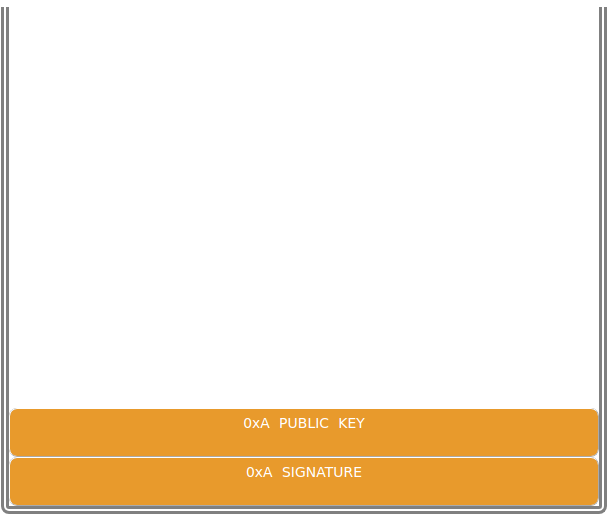
\includegraphics[scale=0.35]{images/script/p2pkh/1.png}
\captionof{figure}{Stato iniziale dello stack.\label{fig:stackp2pkh01}}
\vspace{10pt}
\par}


Incontrato l’operatore OP\_DUP, viene eseguita la copia dell’ultimo valore inserito all’interno dello stack, cioè <A pubkey> come in Figura \ref{fig:stackp2pkh02}.

{\centering
\vspace{15pt}
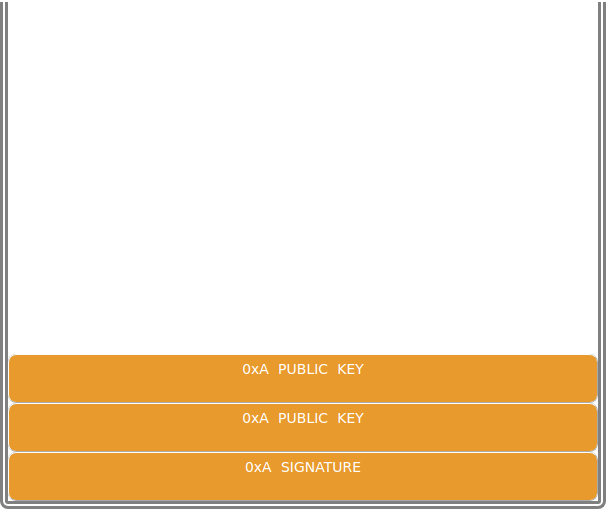
\includegraphics[scale=0.35]{images/script/p2pkh/2.png}
\captionof{figure}{Stato dello stack dopo l’esecuzione dell operatore OP\_DUP.\label{fig:stackp2pkh02}}
\vspace{10pt}
\par}

Incontrando l’operatore OP\_HASH160 viene calcolato l’hash dell’ultimo valore inserito ottenendo lo stato dello stack rappresentato in Figura \ref{fig:stackp2pkh03}.

{\centering
\vspace{15pt}
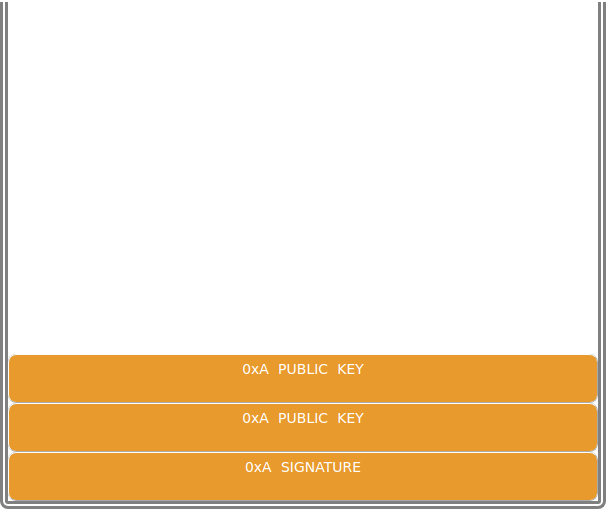
\includegraphics[scale=0.35]{images/script/p2pkh/2.png}
\captionof{figure}{Stato dello stack dopo l’esecuzione dell’operatore OP\_HASH160.\label{fig:stackp2pkh03}}
\vspace{10pt}
\par}

Viene quindi inserito all’interno dello stack l’hash della chiave pubblica atteso, cioè <A Pub Key Hash>, ottenendo lo stack rappresentato in Figura \ref{fig:stackp2pkh04}.

{\centering
\vspace{15pt}
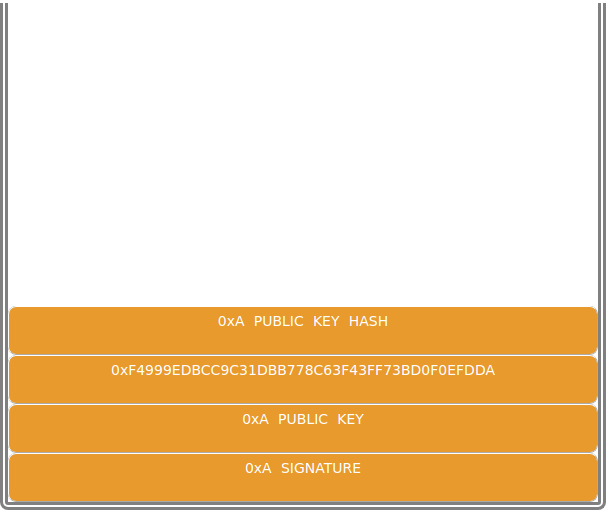
\includegraphics[scale=0.35]{images/script/p2pkh/4.png}
\captionof{figure}{Stato dello stack dopo l’inserimento della chiave pubblica attesa.\label{fig:stackp2pkh04}}
\vspace{10pt}
\par}

L ’operatore OP\_EQUALVERIFY a questo punto verifica che le chiavi pubbliche siano uguali; se lo sono, l’esecuzione continua altrimenti, termina con un risultato diverso da TRUE. Se l’esecuzione prosegue, viene valutato l’ultimo OP code cioè OP\_CHECKSIG, che ha il compito di verificare l’appartenenza della firma e della chiave pubblica alla medesima chiave privata A.

\subsection{P2PK}
Lo script {\it pay-to-public-key \/} è una forma di script più semplice del precedente, perché non viene applicato l’hash alla chiave pubblica e, quindi, l’indirizzo del ricevente è memorizzato nella transazione; per bloccare questo script si necessita solo della firma, il che fa sì che lo stack si semplifichi come segue:
\begin{lstlisting}[language=bitcoinscript, caption={P2PK Script completo.}]
<A Signature>
<A Public Key > OP_CHECKSIG
\end{lstlisting}

Quando il programma viene eseguito, lo stack è popolato con i valori dello script di sblocco come illustrato in Figura \ref{fig:stackp2pk01}.

{\centering
\vspace{10pt}
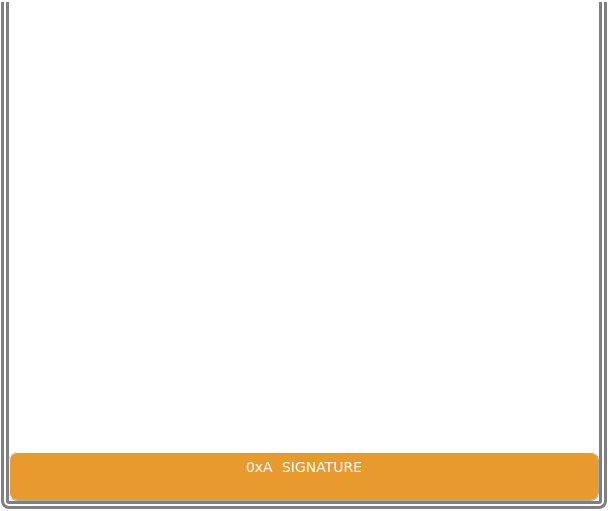
\includegraphics[scale=0.35]{images/script/p2pk/1.png}
\captionof{figure}{Stato dello stack dopo l’inserimento dello scriptSig.\label{fig:stackp2pk01}}
\vspace{10pt}
\par}

Nel passo successivo la chiave pubblica viene inserita nello stack, come rappresentato dalla Figura \ref{fig:stackp2pk02}.

{\centering
\vspace{10pt}
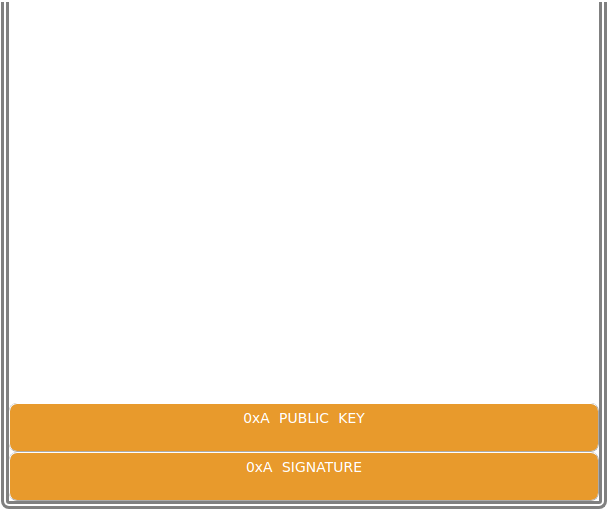
\includegraphics[scale=0.35]{images/script/p2pk/2.png}
\captionof{figure}{Stato dello stack dopo l’inserimento del <public key>.\label{fig:stackp2pk02}}
\vspace{10pt}
\par}

Avviene quindi la verifica tra firma e chiave pubblica con l’operatore OP\_CHECKSIG e, se  l’operatore ha come risultato TRUE, allora la transazione è sbloccabile con lo script di sblocco inserito.\newline
Lo script P2PK, oltre ad essere uno script semplice, viene considerato dagli sviluppatori un errore di implementazione originale, perché non contiene un indirizzo Bitcoin ma contiene la reale chiave pubblica derivata dall’algoritmo di curva ellittica, motivo per cui nell'agosto 2019 da uno script P2PK non è più possibile ricavare un indirizzo Bitcoin tramite il client ufficiale. In Figura \ref{fig:examplep2pkbuild} viene mostrata la differenza del processo di creazione tra uno script P2PK e uno script P2PKH.

{\centering
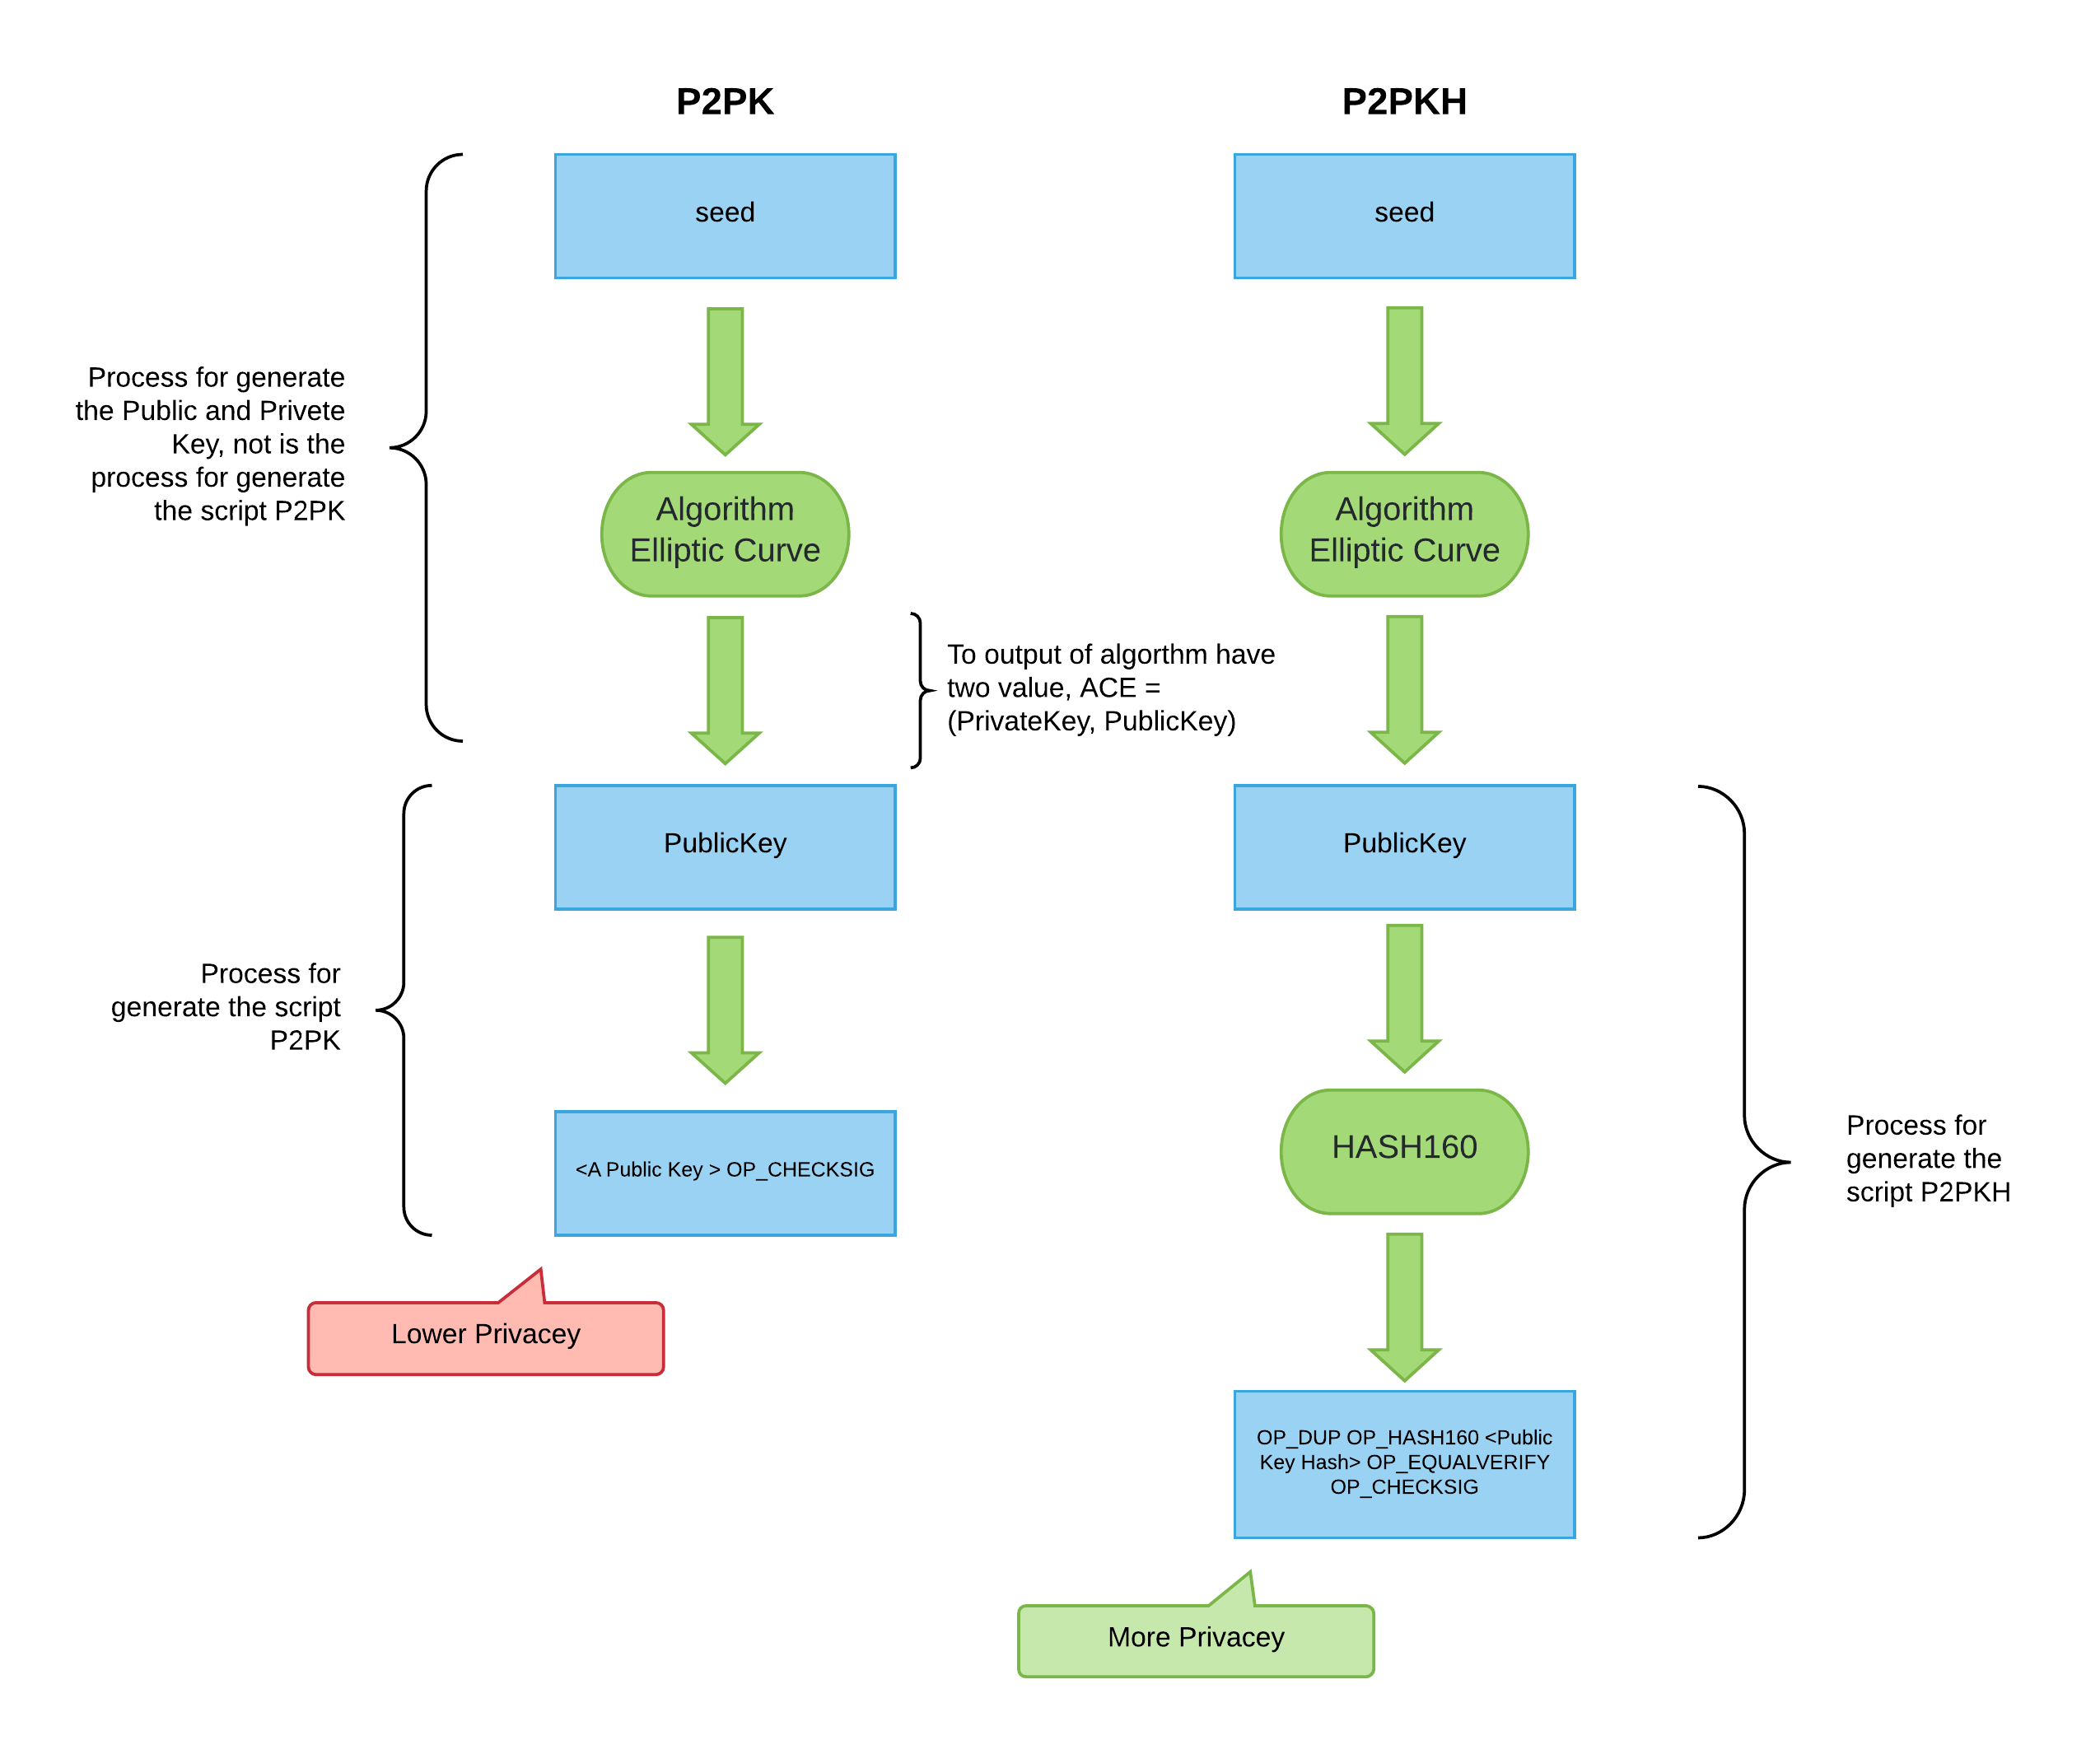
\includegraphics[scale=0.10]{images/proccessBuildP2PK.png}
\captionof{figure}{Rappresentazione del processo di creazione dello script P2PK e P2PKH.\label{fig:examplep2pkbuild}}
\par}

\subsection{P2MS}
\label{sec:p2msbitcoin}
Gli script {\it pay-to-multisignature} definiscono una condizione M:N (molti a molti) dove M è il numero minimo di firme necessarie per verificare lo script di blocco e N è il numero totale di chiavi pubbliche.
Il numero massimo di combinazioni ammesse per uno script P2MS è 15:15, ma solo le combinazioni rientranti nell’intervallo 3:3 sono considerate standard; tutte le restanti combinazioni verranno considerate come non standard.
Un esempio di script P2MS 2:3 è il seguente:

\begin{lstlisting}[language=bitcoinscript, caption={Script P2MS completo.}]
OP_0 <A Signature> <B Signature>
OP_2 <Public key A> <Public key B> <Public key C> OP_3 OP_CHECKMULTISIG
\end{lstlisting}
In questo esempio OP\_0 funge da segnaposto per un bug nell’implementazione di OP\_CHE\-CK\-MULTI\-SIG, il cui unico scopo è quello di aggirare un bug che è diventato accidentalmente una regola di consenso.

Lo stack inizialmente verrà popolato con i valori dello script di sblocco; la presenza dell’operatore OP\_0 implica che lo stack sia vuoto quando lo si incontra. Lo stato dello stack è rappresentato dalla Figura \ref{fig:stackmultsing01}.

{\centering
\vspace{15pt}
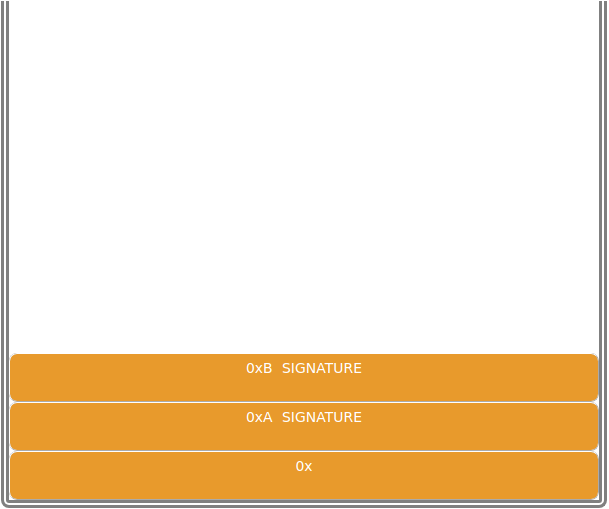
\includegraphics[scale=0.35]{images/script/multisig/1.png}
\captionof{figure}{Stato dello stack dopo l’inserimento dello scriptSig nello stack.\label{fig:stackmultsing01}}
\vspace{10pt}
\par}

L’operatore OP\_2 verifica che nello stack ci siano 2 elementi, successivamente vengono inserite le tre chiavi pubbliche, ottenendo così uno stato come in Figura \ref{fig:stackmultsing02}.

{\centering
\vspace{15pt}
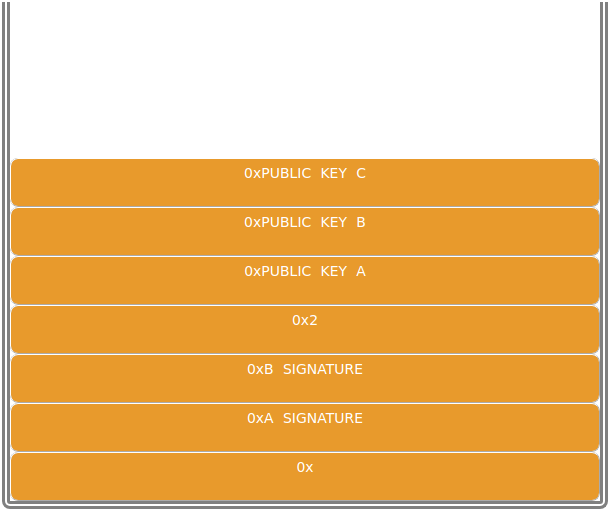
\includegraphics[scale=0.35]{images/script/multisig/2.png}
\captionof{figure}{Stato dello stack dopo la verifica con OP\_2 e l’inserimento nello stack delle chiavi pubbliche.\label{fig:stackmultsing02}}
\vspace{10pt}
\par}

Infine le firme vengono verificate con le chiavi pubbliche mediante l’operatore OP\_CHECK\-MULTI\-SIG in maniera iterativa, cioè la prima firma viene confrontata con tutte le chiavi pubbliche e l’azione si ripete per tutte le firme inserite, come in Figura \ref{fig:stackmultsing03}.

{\centering
\vspace{15pt}
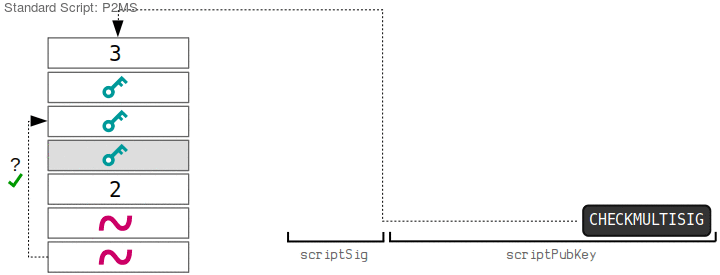
\includegraphics[scale=0.35]{images/script/multisig/3.png}
\captionof{figure}{Esecuzione dell’operatore OP\_CHECKMULTISIG per la verifica delle chiavi \cite{learnmeabitcoin:p2ms}.\label{fig:stackmultsing03}}
\vspace{10pt}
\par}

\subsection{P2SH} \label{sec:p2shBitcoin}
Lo script {\it pay-to-script-hash \/} venne introdotto nel 2012, per semplificare l’uso degli script in transazioni complesse: infatti molto spesso accade di avere script molto grandi, come uno script P2MS 14:15, il che comporta un aumento della complessità dello script di sblocco; la motivazione dell’introduzione dello script P2SH è stata la semplificazione di quest’ultimo, come se fosse un normale pagamento ad un indirizzo Bitcoin.
Questa nuova tipologia semplifica notevolmente lo script di blocco, perché sarà popolato solo dal suo hash, a discapito però dell’aggiunta di una copia dello script di blocco all’interno dello script di sblocco. Si consideri, ad esempio il seguente script P2SH:

\lstinputlisting[label=code:p2shnokey, caption={Script P2SH completo.}]{code/script/p2sh-without-key.btcs}

In questo esempio lo script P2SH (Codice \ref{code:p2shnokey}) completo viene composto dal seguente script di sblocco:
\begin{lstlisting}[language=bitcoinscript, label={code:p2shunlock}, caption={Script P2SH di sblocco.}]
OP_0 <A Signature> <B Signature> OP_2 <Public key A> <Public key B>
<Public key C> OP_3 OP_CHECKMULTISIG
\end{lstlisting}

Esso conterrà anche lo script di blocco, conosciuto, in questo caso, come script di riscatto ({\it redeemScript\/}). Quindi nello script di sblocco si possono distinguere:
\begin{itemize}
  \item {\bf <signature>\/}: Composto da <A Signature> <B Signature>.
  \item {\bf <redeemScript>\/}: Composto da OP\_2 <Public key A> <Public key B> <Public key C> OP\_3 OP\_CHECKMULTISIG.
\end{itemize}

Diversamente, lo script di blocco si semplifica come nell’esempio seguente:
\begin{lstlisting}[language=bitcoinscript, label={code:p2shlock}, caption={Script P2SH di blocco.}]
OP_HASH160 <ScriptSig Hash> OP_EQUAL
\end{lstlisting}

L’esecuzione del Codice \ref{code:p2shnokey} si suddivide in due passaggi:

\begin{enumerate}
  \item Viene valutato lo script di sblocco come descritto nella Sezione \ref{sec:p2msbitcoin}.
  \item Viene verificato l'hash ricavato dallo script di riscatto con l’hash inserito all’interno dello script di blocco.
\end{enumerate}

Il passo 1 dell’esecuzione consiste nella valutazione dello script di sblocco come un normale script P2MS, lasciando invariato lo stato di esecuzione dello stack.
Il passaggio 2, invece, viene eseguito solo se l’esecuzione precedente restituisce TRUE; nel caso di  script P2MS validi l’esecuzione prosegue con una copia dello stack all’interno di un nuovo stack popolato solo dal redeemScript.

Lo stato del nuovo stack viene popolato con i dati relativi allo script di riscatto come mostrato in Figura \ref{fig:stackp2sh01}.

{\centering
\vspace{15pt}
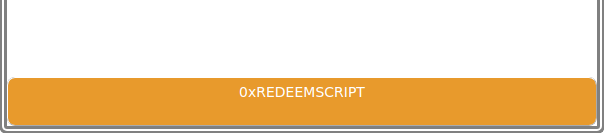
\includegraphics[scale=0.35]{images/script/p2sh/1.png}
\captionof{figure}{Stato dello stack dopo l’esecuzione dello ScriptSig come script P2MS.\label{fig:stackp2sh01}}
\vspace{10pt}
\par}

Viene valutato l’operatore OP\_HASH160, che esegue l’hash del redeemScript e porta lo  stack nello stato riportato in Figura \ref{fig:stackp2sh02}.

{\centering
\vspace{15pt}
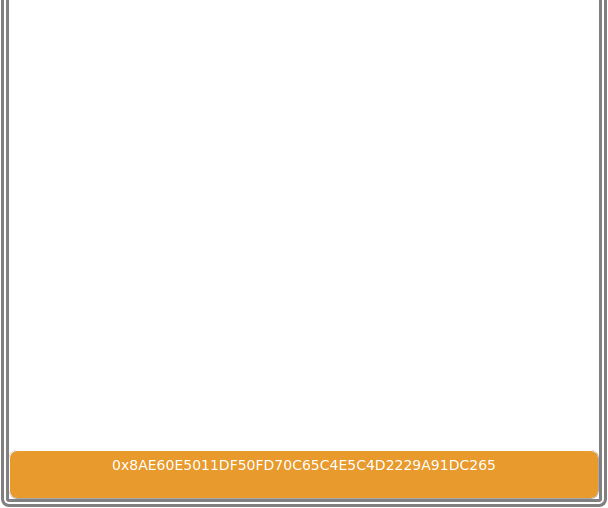
\includegraphics[scale=0.35]{images/script/p2sh/2.png}
\captionof{figure}{Stato dello stack dopo l’esecuzione dell’operatore OP\_HASH160.\label{fig:stackp2sh02}}
\vspace{10pt}
\par}

Come ultimo passaggio viene inserito l’hash atteso contenuto nello script di sblocco, ottenendo lo stato dello stack mostrato in Figura \ref{fig:stackp2sh03}.

{\centering
\vspace{15pt}
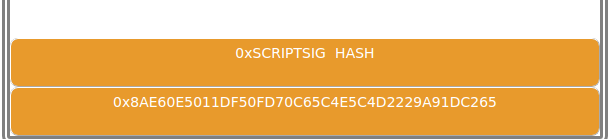
\includegraphics[scale=0.35]{images/script/p2sh/3.png}
\captionof{figure}{Stato dello stack dopo l’inserimento dell’hash atteso.\label{fig:stackp2sh03}}
\vspace{10pt}
\par}

Infine, eseguendo l’operatore OP\_EQUAL viene verificata l’uguaglianza degli hash; l’esito di tale confronto definisce il futuro della transazione.

Nell'implementazione del P2SH è stata aggiunta un’altra importante caratteristica cioè la possibilità di codificare un hash di script come un indirizzo Bitcoin attraverso l’utilizzo della codifica Base58; l’indirizzo ricavato è conosciuto anche come indirizzo P2SH, con l’unica differenza che quest'ultimo inizierà con il numero 3 per convenzione.

Un esempio di indirizzo Bitcoin P2SH:

\begin{lstlisting}[language=bitcoinscript, caption={Indirizzo Bitcoin P2SH.}]
3EBe7iCt2vhC9gqw9UdeaudjYkbfpq3b8c
\end{lstlisting}

Un'indirizzo primitivo Bitcoin:

\begin{lstlisting}[language=bitcoinscript, caption={Indirizzo Bitcoin primitivo.}]
1A1zP1eP5QGefi2DMPTfTL5SLmv7DivfNa
\end{lstlisting}

Attraverso l’indirizzo Bitcoin calcolato dallo script, si può riscrivere il Codice \ref{code:p2shlock} come segue:
\begin{lstlisting}[language=bitcoinscript, label={code:p2shlockwithkey}, caption={Script P2SH di blocco con Indirizzo Bitcoin P2SH.}]
OP_HASH160 <P2SH key> OP_EQUAL
\end{lstlisting}

Quindi lo script completo diventa:

\lstinputlisting[language=bitcoinscript, label=code:p2shkey, caption={Script P2SH completo con indirizzo Bitcoin P2SH.}]{code/script/p2sh-with-key.btcs}

L’esecuzione del Codice \ref{code:p2shkey}, che contiene un indirizzo Bitcoin P2SH al posto del hash dello script, non cambia, perché la chiave ricavata dallo script viene decodificata nel suo hash risultante, così da lasciare la sua esecuzione invariata.
Bitcoin utilizza la convenzione dell'id wallet solo per una semplificazione per l'occhio umano, ma non necessita di queste informazioni per compiere le sue ordinarie operazioni; inoltre gli script P2SH e quindi gli script P2MS (in particolare script P2MS 2:2) vengono utilizzati estensivamente per la creazione e la gestione di canali all’interno della tecnologia {\it Lightning network\/}, che aumentano drasticamente la velocità delle transazioni con Bitcoin, utilizzando un protocollo {\it off-chain\/}.

\subsection{Transazioni null data (OP\_RETURN)}\label{sub:sectionNUllaDataScript}
La blockchain di Bitcoin e, più in generale, le tecnologie blockchain hanno potenziali usi ben oltre i pagamenti. Molti sviluppatori hanno tentato di utilizzare Bitcoin script, per sfruttare la sicurezza e la resilienza del sistema, per applicazioni quali servizi notarili digitali, certificati azionari e {\it smart contract\/}.

I primi tentativi di utilizzare il linguaggio di script di Bitcoin per questi scopi hanno comportato la creazione di output di transazioni, che registravano dati sulla blockchain; nella versione 0.9 di Bitcoin core del 2014, è stato aggiunto un nuovo tipo di operatore chiamato OP\_RETURN che marca la transazione come non correlata ad un movimento di bitcoin, ma ad un'archiviazione di dati. Questo operatore ha permesso ai miner di identificare la transazione e decidere se validarla o meno, considerando il problema che, archiviando una transazione con uno script non valido, oltre a creare un UTXO non spendibile, lo spazio richiesto della blockchain di bitcoin sarebbe aumentato, aumentando quindi anche le commissioni richieste dal miner.
Per aggirare questo problema, il team di sviluppo decise di limitare la porzione di dati a 80 byte.

\begin{lstlisting}[language=bitcoinscript, label={code:nulldata}, caption={Uso dell'operatore OP\_RETURN.}]
OP_RETURN <data>
\end{lstlisting}

Lo script precedente non fa altro che marcare il campo <data> come dati grezzi che non riguardano una transazione; infatti la semantica dell’operatore OP\_RETURN marca la transazione come invalida, quindi i dati non vengono valutati.

\section{Mining}
\label{sec:miningbitcoin}

Il processo di Mining si avvale dell’algoritmo di Proof of Work, per generare nuovi bitcoin e proteggere la rete da attacchi di malintenzionati, come ad esempio la pubblicazione di un blocco non valido o la modifica di una transazione all’interno di un blocco.\newline
Bitcoin esegue la validazione delle transazioni in media ogni 10 minuti ed esse vengono considerate valide solo quando il blocco che le contiene viene accodato alla catena ufficiale; ogni transazione può includere all’interno un valore di bitcoin che equivale ad una tassa indirizzata al miner per ricompensa del lavoro svolto, il quale può scegliere di dare precedenza a transazioni con una commissione maggiore di un quantitativo di bitcoin a loro scelta.\newline
Bitcoin stabilisce un processo di creazione di nuova moneta decrescente e limitato: infatti impone un limite superiore massimo di \(2.1 * 10^{15} \) bitcoin; il valore creato dai miner si dimezza ogni 210.000 blocchi, in media ogni 4 anni.
La creazione di bitcoin iniziò con un ammontare pari a 50 bitcoin per blocco nel gennaio 2009 e si dimezzò a 25 bitcoin nel novembre 2012, stimando così l’emissione completa di tutti i bitcoin disponibili nel 2140; al termine dell’emissione, il guadagno di ogni miner sarà esclusivamente il valore della commissione.
L’utilizzo dell protocollo Proof of Work, che è per sua natura {\it CPU-bound\/}, nel corso degli anni, con l’aumentare della competitività nel settore del mining di bitcoin, portò ad un aumento esponenziale della potenza di hashing, subendo così un cambiamento radicale della tecnologia utilizzata: si è passati da comuni CPU a componenti appositi per il calcolo della funzione hash del tipo FPGA (\emph{mining and field programmable gate array}).\footnote{Nel 2014, l'energia consumata dalla rete Bitcoin era pari al consumo di elettricità dell'Irlanda (O'Dwyer e Malone, 2014)}
L’aumento della potenza di hashing (Figura \ref{fig:hashrate}) portò anche ad un aumento della difficoltà di estrazione di un blocco conosciuta come difficoltà metrica (Figura \ref{fig:metrix}).

{\centering
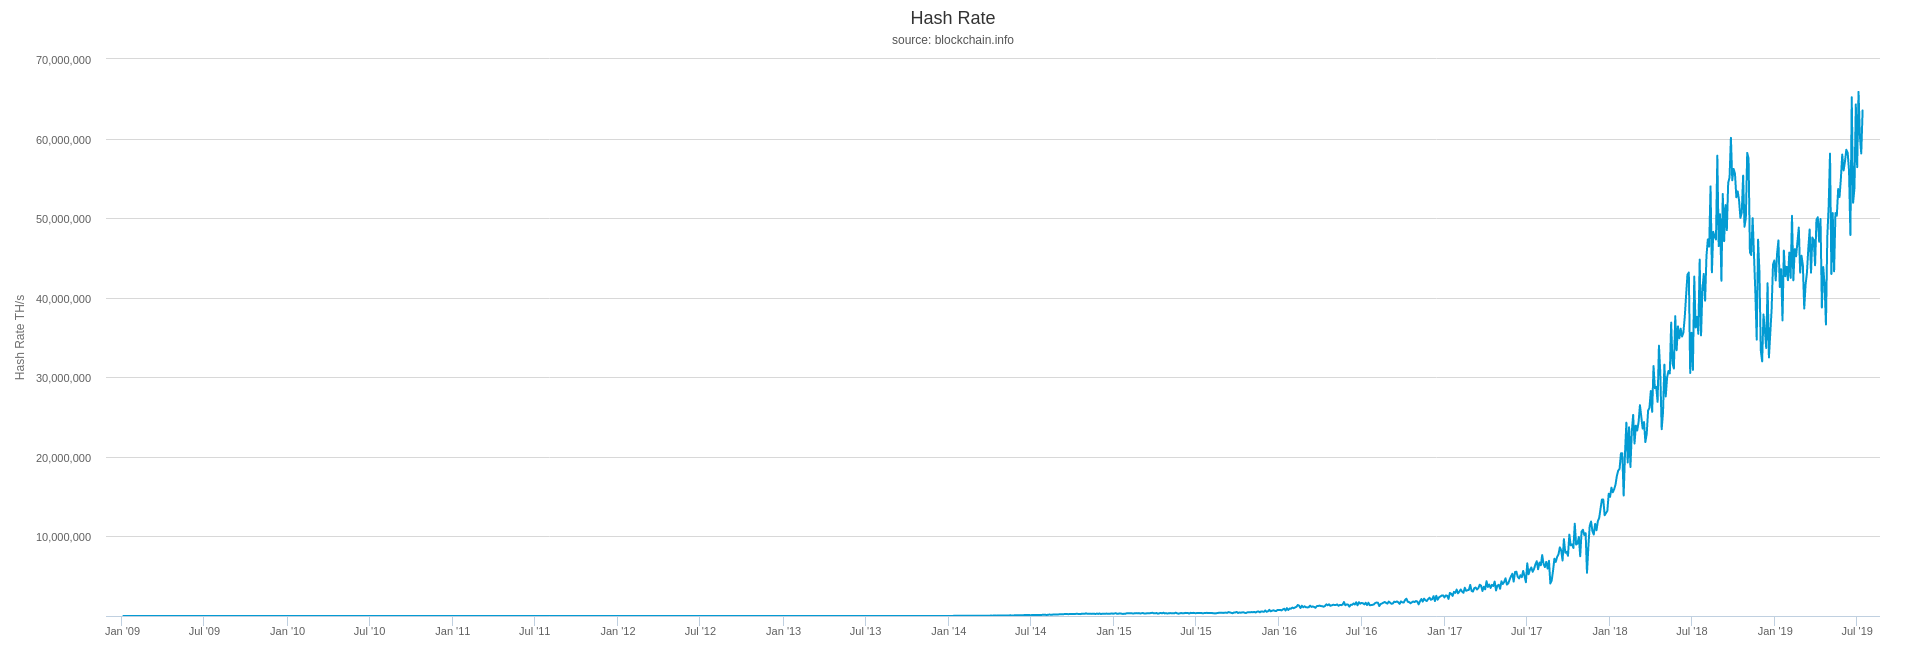
\includegraphics[scale=0.2]{images/hash-rate.png}
\captionof{figure}{Grafico della crescita della potenza di hashing in data 28/09/2019. Fonte: blockchain.com.\label{fig:hashrate}}
\par}

{\centering
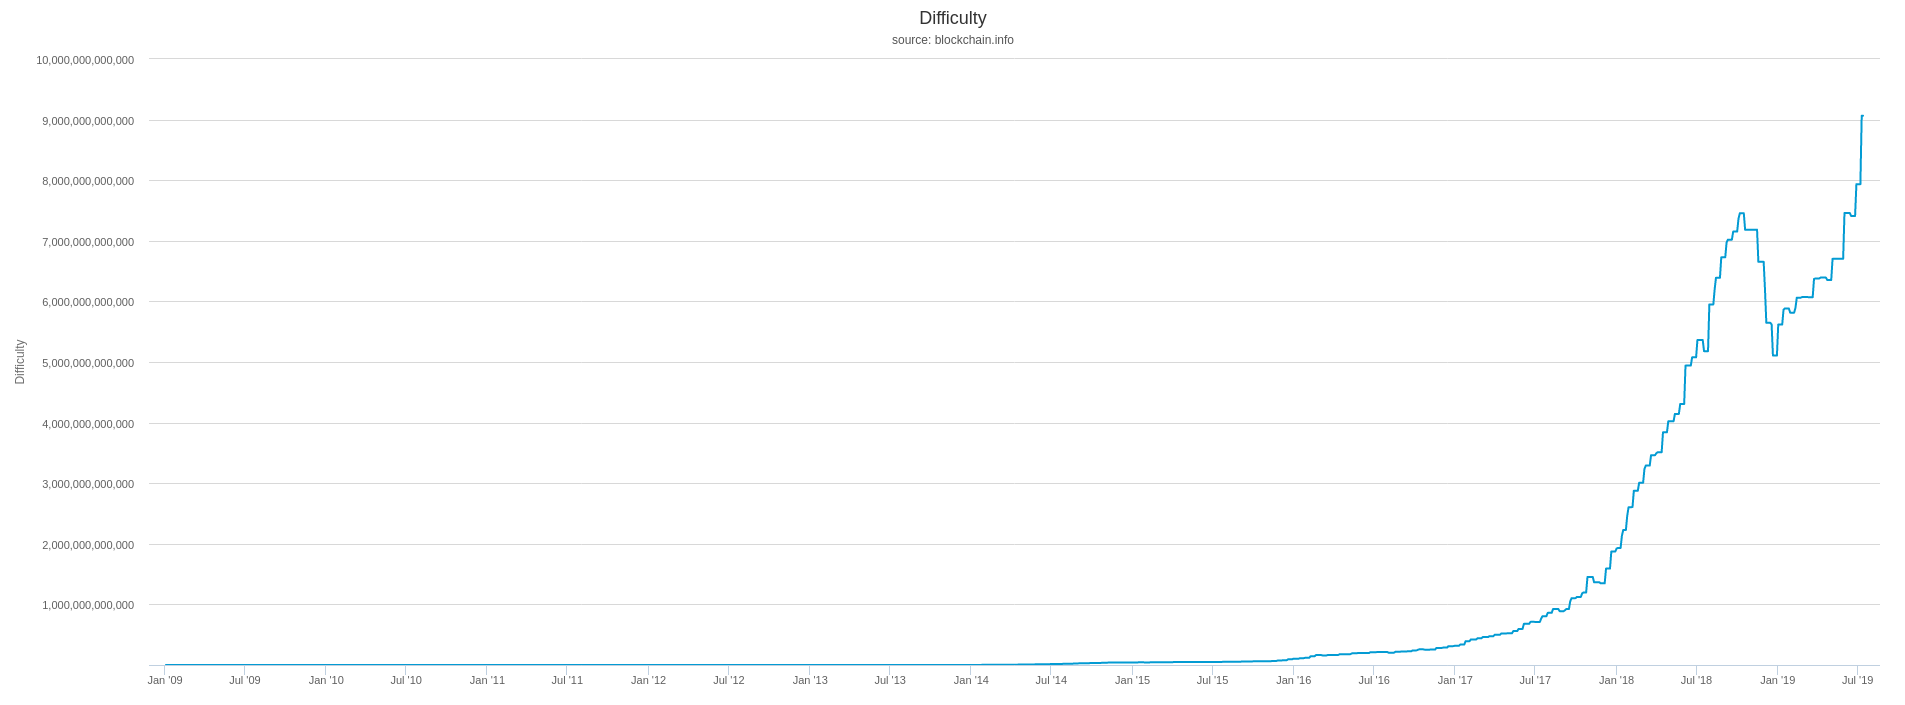
\includegraphics[scale=0.2]{images/difficulty.png}
\captionof{figure}{Grafico della crescita della difficoltà metrica in data 28/09/2019. Fonte: blockchain.com.\label{fig:metrix}}
\par}
